% 装配
%作者:赵启
%上次更新:2020年1月10日 17:20

\chapter{零件的选择、加工与机构装配}

\section{零件材料的选择及加工}

\subsection{材料的选择}

{\songti 工欲善其事,必先利其器。在整个加工与装配过程中,我们分别根据基座、三臂与机械手
的加工零件选择进行了详细的探讨。
我们在首先确定了材料选择,其中机械手的部分由于设计个性化较强且结构复杂,因此我们采用了
光敏树脂进行3D打印;对于基座和臂的部分,我们选择了亚克力板进行零件制作。
对于传动和紧固件,如蜗轮蜗杆、轴等零件我们使用了生产加工中最常用的碳素结构钢——
45号钢进行加工。}

\subsection{零件的加工}

{\songti 在加工的过程中,我们实行了三步走战略——第一步,有标准件的直接购买标准件;
第二步,能利用学校学生创新中心资源进行自主加工的,尽量自己加工;第三步,如果自己
加工满足不了公差要求、方法困难、缺少设备或者有较高的危险性,我们会联系淘宝或者交
大附近的加工厂进行加工。}

{\songti 第一步,对于标准件的使用,我们首先充分利用了工训的各种已有资源,如连接
和紧固用的螺钉螺栓,这对于我们节省成本提供了很大的帮助;而对于能使用标准件的部分,
如带传动、蜗轮蜗杆传动、电机以及轴承等,我们都尽可能地选用了标准件。}

{\songti 第二步,对于自己可以进行加工的零件,我们利用学生创新中心的设备进行了一
系列加工——使用钻床进行亚克力板的钻孔、使用普通车床进行轴和蜗杆的加工与倒角,使用人力
锯进行轴的切割、使用激光切割机进行10mm以下亚克力板的切割、使用锉刀进行孔径和轴肩的
微调,使用3D打印机进行手部零件的打印。这一部分对于我们的动手能力有了很大的提升,也
很好地利用了周围的资源,节约了很大一部分加工成本。}

{\songti 第三步,委托校外相关厂商加工零件。由于现实条件的约束与加工需求之间的矛盾,
我们对于无法利用学校资源加工的一些零件,委托给了淘宝与阿里巴巴加工商或者是灯辉路的
上海银燕光电仪器厂进行加工,其中包括20mm厚亚克力板的切割、亚克力板的铣削、蜗杆的
数控车床加工、厚齿轮与带轮的开键槽、公差要求较高的轴与杆的加工、材质要求较高的手部
3D打印件的制作等等。}


\subsection{加工中遇到的问题及解决方法}

{\songti 万事开头难,在准备的过程中我们也难免遇到了各式各样的困难与问题。}

{\songti 一,对于采用了就使用碳纤维板和亚克力板作为
主要材料进行了讨论,后来经过与商家联系得知使用碳纤维板进行加工的预算是使用亚克力
板的五倍,远远超出了我们的总预算,并且亚克力板的强度与加工性也已经满足我们的加工
需求,因此我们最终选择了亚克力板。}

{\songti 二,对于手部构件的3D打印,我们发现学校的3D打印机打印出来的产品表面粗糙,
与我们进行食品夹取的需求的不符,因此我们将与食物接触的部分委托给了校外厂商进行3D打印。}

{\songti 三,由于我们很多零件需要开键槽,如蜗杆、轴、手部齿轮,但学生创新中心又
没有相应的插床设备,因此我们更改了设计,并且联系了剑川路地铁站附近的上海银燕光电仪器厂进行加工。}

{\songti 四,由于学生创新中心不能切割10mm以上的亚克力板,且无法对其进行铣削,而我们
的设计中大臂的厚度是20mm厚且需要铣削以配适电机,所以我们联系了郑州的一家加工厂进行了
相应的亚克力板的加工。}


\section{机构的装配}

\subsection{基座的装配}

\subsubsection{基座装配过程}

{\songti 对于基座的装配,由于蜗杆与轴承之间是过盈配合,所以我们首先进行了86支架、
轴承固定架与6003轴承的配合,再将车削加工号的蜗杆与轴承配合,再安装底座电机和联轴器,将这
部分构件装配完成后一起固定在已经打好孔的定位底板上,最后从下到上安装轴承垫片、推力
轴承和底基座涡轮。}

\begin{figure}[!htp]
    \centering
    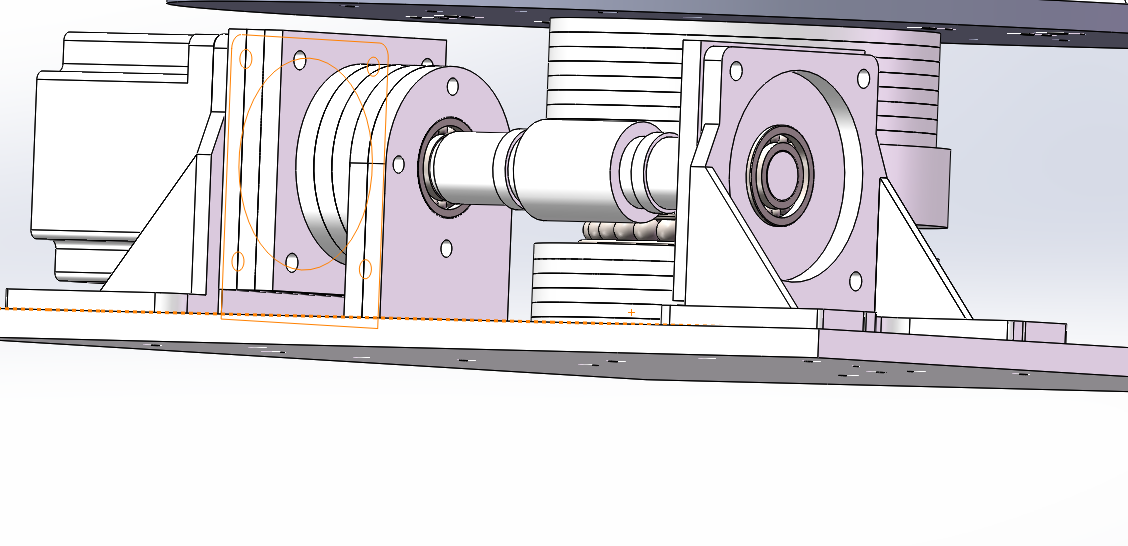
\includegraphics[width=12cm]{Assembly_drawing.png}
    \bicaption[基座装配图]{基座装配图}{Assembly drawing of foundation}
    \label{fig:基座装配图}
\end{figure}

\subsubsection{遇到的问题及解决方法}

{\songti 装配基座的过程中,我们遇到的最大的问题就是上方云台的螺栓在进行旋转时
会与基座上的电机相撞,导致无法进行360°周转,甚至会引起联轴器的损坏。但是我们发现
学生创新中心提供的M5螺栓只有30mm和40mm两种规格,使用30mm螺栓太短而无法完成装配,
而使用40mm螺栓会过长而导致上述的干涉问题。因此我们决定使用手工锯将40mm螺栓锯断
成36mm的非标准件,从而满足了我们的装配需求。}

{\songti 因为我们装配40mm螺栓时使用了防松螺母,且底座位置很低,因此我们在重新更新
螺母时花费了很大的人力功夫,这也是给了我们一个惨痛的教训——事无巨细,以后装配前也要
考虑好螺栓等小零件的干涉问题,不能图快而事倍功半。}


\subsection{机械臂的装配}

\subsubsection{机械臂装配过程}

{\songti 由于机械臂比较复杂,我们采用了从部分到整体,从难安装到易安装的顺序逐步
装配的。对三段臂先进行分别的组装,安装上相应的轴承、转轴、心轴、电机、带轮
与同步带、涡轮和蜗杆以及联轴器,再按照从下到上的顺序逐节装配,在两侧加上肋板,
使用螺母和螺栓进行最终的固定。}

\begin{figure}[!htp]
    \centering
    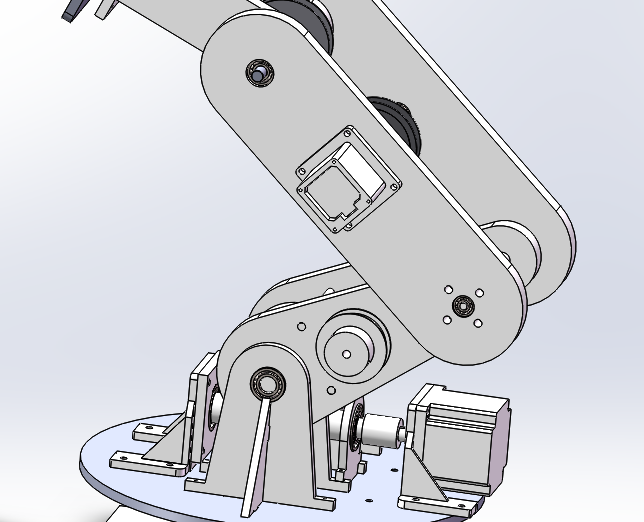
\includegraphics[width=12cm]{Robot_arm_assembly_drawing.png}
    \bicaption[机械臂装配图]{机械臂装配图}{Assembly drawing of mechanical arm }
    \label{fig:机械臂装配图}
\end{figure}

\subsubsection{遇到的问题及解决方法}

{\songti 在机械臂的装配过程中,我们也需要了很多问题。首先是装配顺序的问题,
由于我们首先进行了两个大臂的装配,发现电机受力很大,于是就在大臂上进行打孔
,用心轴进行分担受力和弯矩。但由于重新拆装添加心轴十分麻烦,我们就利用手动
车床对心轴进行了车削加工,从而顺利完成了装配;在进行机械臂整体装配的过程中,
我们发现由于上方整体重力过大而导致云台上方固定部分容易侧翻,因此我们又为支座
添加了角铁,最终得以紧固;在委托厂商进行加工的时候,我们也没有为亚克力板的切割
提供公差余量,因此在安放轴承和电机的时候绝大部分都是过盈配合,我们通过锉刀进行了
扩孔、通过车床减小了轴的直径,完成了过盈配合。}

\subsection{机械手的装配}

\subsubsection{机械手装配过程}

{\songti 对于机械手的装配,我们也是根据从难到易的顺序,先安装最难进行配合的,
再对较易配合的逐步安装,从而有一马平川的效果。先是将机架横板与齿轮、电机进行配合,
再通过深沟球轴承安装伞齿轮,最后完成机架竖板和机械爪各配件之间的装配。}

\begin{figure}[!htp]
    \centering
    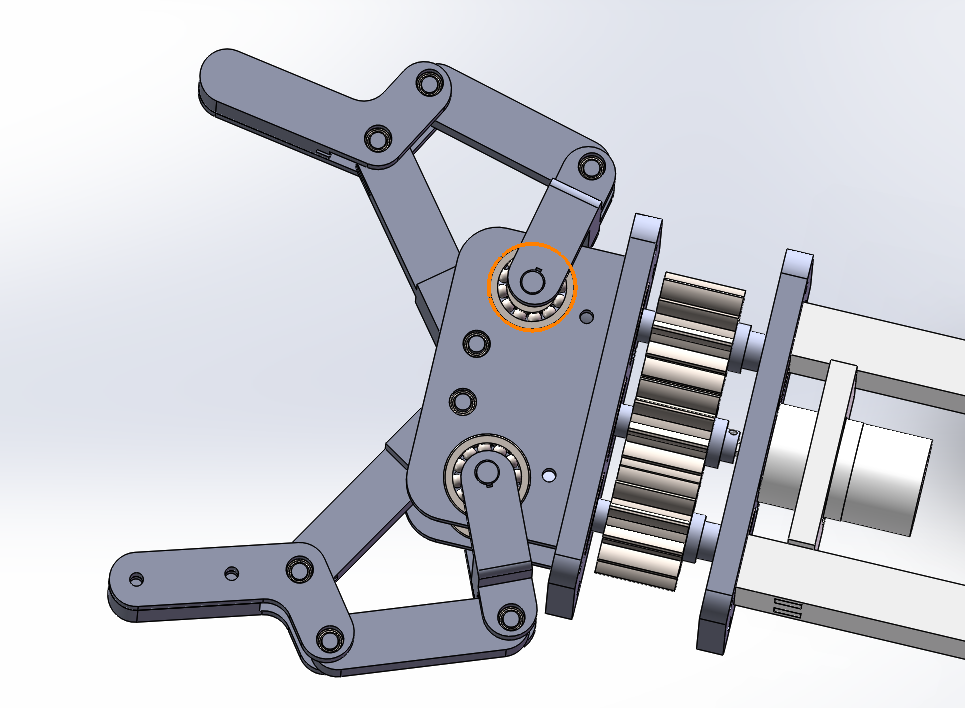
\includegraphics[width=12cm]{Robot_assembly_drawing.png}
    \bicaption[机械手装配图]{机械手装配图}{Assembly drawing of manipulator}
    \label{fig:机械手装配图}
\end{figure}

\subsubsection{遇到的问题及解决方法}

{\songti 在机械手的装配过程中,我们发现3D打印并不能很好的生成螺纹,于是我们利用
直径略大的螺栓进行了旋转配合,由于3D打印件塑性很高,因此在配合的过程中自己形成了
螺纹纹路。在进行直齿轮和伞齿轮轴的配合中,我们发现键槽由于较小而不需要键连接就能
完成过盈配合,因此也进行了直接配合的改进策略。}
